%\documentclass{article}
%
%\usepackage [spanish] {babel} 
%\usepackage [T1]{fontenc}
%\usepackage [latin1]{inputenc}
%\usepackage{amsthm}
%%\usepackage{algorithmic}
%\usepackage{algorithm}
%\usepackage{algpseudocode}
%\usepackage{graphicx}
%\usepackage{epstopdf}
%
%\title{TP2 Ej.1 Descripci\'on del algoritmo} 
%\author{Mat\'ias Chapresto \\ Nicol\'as Dato \\ Ezequiel Fattori \\ Silvio Vileri\~no}
%\newtheorem{Ejemplo}{Ejemplo}
%%\renewcommand{\algorithmicprint}{\textbf{function}}
%
%\begin{document}
%
%\maketitle

\subsection{Descripci\'on del problema}
El problema consiste en modelar un juego de roban\'umeros en el cual ambos jugadores juegan empleando la estrategia \'optima. El juego consiste en una serie de cartas con valores enteros que los jugadores deben ir robando por turnos. Solo se puede robar una serie de cartas que sean contiguas y que comiencen por alguno de los extremos. El jugador que obtenga una suma mayor gana.
El algoritmo debe calcular, a partir de una tanda de cartas, como van a ser las jugadas de ambos jugadores en cada turno, suponiendo que ambos jugadores juegan de "forma \'optima", es decir, de manera de maximizar la diferencia final a favor suponiendo que el contrincante har\'a lo mismo cuando sea su turno.
En la figura 1 se muestran ejemplos del problema junto con parte de su soluci\'on. Los turnos del primer jugador est\'an en rojo y los del segundo jugador en azul.

\begin{figure}[h]
\centering
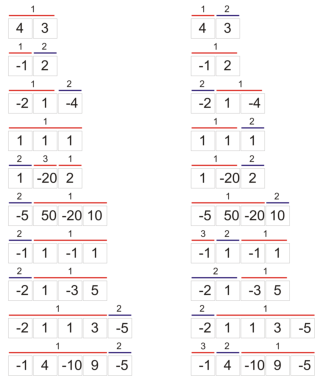
\includegraphics{cartas.png}
\caption{Soluciones \'optimas del juego (izquierda) y no \'optimas(derecha).}
\end{figure}

\subsection{Descripci\'on del algoritmo}
Este problema presenta una estructura recursiva. Cada vez que un jugador hace su jugada, el problema queda reducido a una instancia mas peque\~na del mismo, en la cual el jugador que comienza es el otro. La estrategia para resolverlo es programaci\'on din\'amica.\\
\\
Se llamar\'a $ A_{i}$ a la tira de n\'umeros inicial, con la que el juego comienza. Tambi\'en se define, coloquialmente, el t\'ermino "juego \'optimo" para referirse al desarrollo de un juego en el cual cada jugador juega seg\'un la estrategia dada por el enunciado. Esta estrategia es: jugar en cada jugada de manera de maximizar la diferencia de puntos a favor, suponiendo que el otro jugador en cada jugada har\'a lo mismo. El "juego \'optimo" queda entonces definido recursivamente a partir del caso base: un juego que comienza con una \'unica ficha, que solo puede jugarse de una manera (el primer jugador agarrando esa ficha).\\
\\
Se definen las siguientes funciones:\\
$$S(i,j)=\sum_{i \le k \le j} A_{k}$$
$$P(i,j,h)= p1 - p2$$
Donde $p1$ y $p2$ son los puntajes sumados por los jugadores 1 y 2 respectivamente, luego de jugar \'optimamente la subinstancia dada por la subtira $A_{k} ; i \le k \le j $, comenzando por el jugador $h$ (jugador1 = 1, jugador2 = -1).\\
\\
El algoritmo se divide en tres partes:\\
\\
\underline{Parte 1:} Se calcula la funci\'on $S$. Se hace por programac\'ion din\'amica guardando en una tabla los valores $S(i,j)$ y usando la f\'ormula de recursi\'on $$S(i,j) = S(i,j-1) + A_{j}.$$ (con $S(i,i-1)=0$).\\
\begin{algorithmic}
\For {i=1 to n}
	\For {j=i to n}
		\State $S(i,j) = S(i,j-1) + A_{j}$ 
	\EndFor
\EndFor
\end{algorithmic}
\underline{Parte 2:} Se calcula la funci\'on P, tambi\'en por programaci\'on din\'amica, usando la $S$ ya calculada. Se guarda en una tabla $P(i,j,1)$, pudiendo calcularse $P(i,j,-1) = -P(i,j,1)$ a partir de \'esta. La regla de recursi\'on es:
$$P(i,j,1) = max \{ \ max\{ S(i,k) + P(k+1,j,-1) \ | \  i \le k \le j \} , max\{ S(k,j) + P(i,k-1,-1) \ | \ i \le k\le j \} \ \}$$ con $P(i,i-1,-1) = 0$.\\
\\
Ya que la recursi\'on requiere para el c\'alculo de $P(i,j)$ el c\'alculo de $P(i,j') ; j' \le j$ y de $P(i',j) ; i' \ge i$ la tabla se calcula entonces de menor a mayor en las columnas, y por cada columna de mayor a menor en las filas.\\
La tabla contiene en el lugar $(i,j)$ la tupla $(res(i,j),P(i,j))$ donde $res(i,j)$ son los indices que limitan la subtira que queda por jugar despues de jugar la subtira $(i,j)$. Si ya no se juega mas, $res(i,j)=(0,0) $.\\

\begin{algorithmic}[1]
\For {j=1 to n}
	\For {i=j to 1}
		\State $MAX = -\infty$
		\For { k =i-1 to j}
			\If { $S(i,k) + P(k+1,j) > MAX$ }
				\State $MAX \leftarrow S(i,k) + P(k+1,j)$
				\If { $k \neq j$ }
					\State $res(i,j) \leftarrow (k+1,j)$
				\Else
					\State $res(i,j) \leftarrow (0,0)$
				\EndIf
			\EndIf
		\EndFor

		\For { k = j+1 to i}
			\If { $S(k,j) + P(i,k-1) > MAX$ }

				\State $MAX \leftarrow S(k,j) + P(i,k-1)$
				\If { $k \neq i$}
					\State $res(i,j) \leftarrow (i,k-1)$
				\Else
					\State $res(i,j) \leftarrow (0,0)$
				\EndIf
			\EndIf
		\EndFor
	\EndFor
\EndFor
\end{algorithmic}

\underline{Parte 3:} Se calcula, a partir de las tablas ya calculadas, el desarrollo del juego a partir de su instancia inicial. Se guarda la cantidad de turnos jugados y las fichas robadas por izquierda o derecha en cada turno.

\begin{algorithmic}
\State var $turno \leftarrow 1$
\State var $puntj1 \leftarrow 0$
\State var $puntj2 \leftarrow 0$
\State var $i \leftarrow 1$
\State var $j \leftarrow n$
\State var $jugadas(lado,cant)$
\Loop
	\If{$turnos = impar$}
		\State $puntj1 \leftarrow puntj1 + puntoslevantados$
	\Else
		\State $puntj2 \leftarrow puntj2 + puntoslevantados$ 
	\EndIf

	 \If{$levantoporizq$}
		\State $jugadas.lado[turno-1] \leftarrow izq$
		\State $jugadas.cant[turno-1] \leftarrow cantcartaslevantadas$
	\Else
		\State $jugadas.lado[turno-1] \leftarrow der$
		\State $jugadas.cant[turno-1] \leftarrow cantcartaslevantadas$
	\EndIf
	
	\If{$res(i,j)=(0,0)$}
		\State break
	\EndIf
	\State $(i,j) \leftarrow res(i,j)$
	\State $turno \leftarrow turnos+1$
\EndLoop
\end{algorithmic}
Donde $puntoslevantados$, $cantcartaslevantadas$ y $levantoporizq$ se obtienen como funci\'on $O(1)$ de $res(i,j)$, y no se explicitan para simplificar la exposici\'on. Las variables $puntj1$, $puntj2$, $turno$ y $jugadas$ se usan luego para construir la salida.

\subsection{Correctitud del algoritmo}
A continuaci\'on se da una demostraci\'on de por qu\'e la estrategia elegida cumple el requerimiento del enunciado. Este requerimiento es: "maximizar la diferencia de puntos a favor al final del partido, asumiendo que el otro jugador tiene la misma estrategia".\\
La estrategia elegida es: para cada posible tira que se puede extraer, calcular la suma de los n\'umeros de la tira y sumarle la diferencia que se consigue a favor al jugar de forma \'optima durante el resto del juego (que ya est\'a definida por ser el resto del juego una instancia m\'as peque\~na). Extraer la tira que maximice este n\'umero.\\
Sea entonces $A_{k}$ una tira inicial de cartas. Si $A_{k}=(c1)$ hay una \'unica manera de jugar, y por lo tanto la estrategia cumple el requerimiento. Sup\'ongase que la estrategia cumple el requerimiento si $A_{k}$ es de longitud $\le m$. Para $A_{k}$ de longitud $m+1$, una forma gen\'erica de jugar el juego es una elecci\'on de cartas a robar inicialmente, de puntuaci\'on total $S$, seguida de un cierto desarrollo en el cual la diferencia conseguida a favor es $P$. Ll\'amese $P'$ a la diferencia a favor conseguida como resultado de jugar \'optimamente el juego que comienza a partir de la primer elecci\'on de cartas (comenzado por el jugador2). Por hip\'otesis inductiva se cumple que $P \le P'$ luego la diferencia a favor obtenida en este juego es $S+P \le S+P'$. Adem\'as, por definici\'on, $S+P' \le M$ donde $M$ es la diferencia a favor que se consigue haciendo la primer elecci\'on seg\'un la estrategia, y jugando \'optimo durante el resto del juego.\\
\\
 Por \'ultimo resta ver que esta estrategia se traduce formalmente en la recursi\'on dada para $P(i,j,h)$ en la descripci\'on del algoritmo, pero esto es muy f\'acil de ver por inducci\'on y no se escribe.\\
\\
\subsection{Complejidad}
La parte 1 del algoritmo es $O(n^{2})$, ya que son 2 bucles for anidados con interior $O(1)$ con a lo sumo $n$ iteraciones cada uno.
La parte 2 del algoritmo es $O(n^{3})$ ya que son 2 bucles for anidados con a lo sumo $n$ iteraciones cada uno, y dentro de ellos hay dos bucles for sucesivos, cada uno de ellos $O(n)$.
La parte 3 del algoritmo es O(n) ya que el loop se ejecuta a lo sumo tantas veces como la cantidad de turnos, que es a lo sumo $n$, y el interior del loop es $O(1)$.\\
Por lo tanto el tiempo total del algoritmo es $O(n^3)$

\subsection{C\'odigo fuente}
Ver Ap\'endice.

\subsection{Verificaci\'on}
Para la verificaci\'on se emplearon las mismas instancias que fueron dadas como ejemplo del problema y su resoluci\'on. \'Estas fueron calculadas a mano, y luego se verific\'o que efectivamente el algoritmo daba el mismo resultado (la misma diferencia de puntos a favor) en cada caso.

\subsection{An\'alisis de performance}
La segunda parte del algoritmo, el c\'alculo de la tabla $P$, es de complejidad $O(n^3)$ y se lleva la mayor parte del tiempo de ejecuci\'on para $n$ grande.
El c\'alculo de esta tabla, que tiene $n^2/2$ posiciones, involucra para cada posici\'on el c\'alculo del m\'aximo de una cantidad de elementos que depende \'unicamente de la posici\'on que se c\'alcula, no del contenido de las cartas. Como el tiempo que demora el algoritmo est\'a dominado por esta parte, es de esperar que el contenido de las cartas no cambie apreciablemente los tiempos de ejecuci\'on. \'Esto se puede constatar por medio de la experimentaci\'on.\\
\\
Se hizo una experimentaci\'on con tama\~nos n de entrada entre 100 y 400. Se distingui\'o la distribuci\'on de los valores de las cartas en tres casos : uniforme en $[-50;50]$, uniforme en $[-100;0]$ y uniforme en $[0;100]$. Todos los casos dieron tiempos similares. En la gr\'afica puede observarse una curva similar a las de la forma $ax^{m}$. Se puede comprobar que al variar de $n=200$ a $n'=300$, $n'=(3/2)n$, el tiempo pasa de un promedio de $200$ a un promedio de $650 \sim 200.(3/2)^3$. \'Esto comprueba que la curva es c\'ubica.
En el ap\'endice se adjuntan las gr\'aficas experimentales de $tiempo(n)$.

%\end{document}
